%!Tex Root = ../main.tex
% ./Packete.tex
% ./Design.tex
% ./Deklarationen.tex
% ./Aufgabe1.tex
% ./Aufgabe2.tex
% ./Aufgabe3.tex
% ./Aufgabe4.tex
% ./Appendix.tex

\section{General Information}

\begin{frame}{General Information}{Organsiation}
  \begin{itemize}
    \item there will be a \alert{cheatsheet}:
      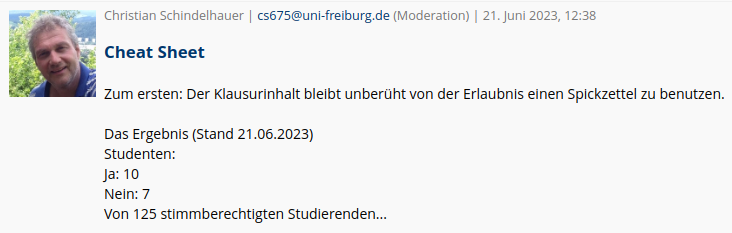
\includegraphics[width=0.8\textwidth]{./figures/forum.png}
  \end{itemize}
\end{frame}
